\documentclass{article} % For LaTeX2e
% We will use NIPS submission format
\usepackage{nips13submit_e,times}
% for hyperlinks
%\usepackage{hyperref}
\usepackage{url}
% For figures
\usepackage{graphicx} 
\usepackage{subfigure} 
% math packages
\usepackage{amsmath}
\usepackage{amsfonts}
\usepackage{amsopn}
\usepackage{ifthen}
\usepackage{natbib}
\usepackage{color}
\usepackage{float}
\usepackage{placeins}
\usepackage{geometry}
\usepackage{listings}

\title{Project-II by Group Istanbul}

\author{
Johan Droz\\
EPFL \\
\texttt{johan.droz@epfl.ch} \And
Arseniy Zaostrovnykh\\
EPFL \\
\texttt{arseniy.zaostrovnykh@epfl.ch}
}

% The \author macro works with any number of authors. There are two commands
% used to separate the names and addresses of multiple authors: \And and \AND.
%
% Using \And between authors leaves it to \LaTeX{} to determine where to break
% the lines. Using \AND forces a linebreak at that point. So, if \LaTeX{}
% puts 3 of 4 authors names on the first line, and the last on the second
% line, try using \AND instead of \And before the third author name.

\nipsfinalcopy 

\newcommand{\todo}[1]{}
\renewcommand{\todo}[1]{{\color{red} TODO: {#1}}}

\begin{document}

\maketitle

\begin{abstract}
In this report we describe our results for the second project of the 2015 PCML class.
Our goal is to design a system that, given an image, is able to recognize three kinds of object in it.
To achieve this, we experimented with several Machine Learning methods: SVM, Random Forests and Neural Networks. Each method was individually tuned to improve its performance, and finally we tried to improve the accuracy of the system by combining different methods.

\end{abstract}

\section{Introduction}

The problem of classifying images is a hot topic on which most of the big IT companies are working.
Google\cite{GoogleCar}, Tesla\cite{TeslaAutopilot} and probably other companies are building an autonomous car. It has to be able to recognize in real-time objects such as other vehicles, pedestrians, traffic lights, roadsigns etc.
Every day on social networks, millions of images are uploaded, processed and classified\cite{facebook}. Human and face recognition applied to these images improves personal experience. 

The system we have to design is simpler than the previous examples because we are restricted only to 4 categories of objects. Nevertheless, the task of recognizing an object in an image is still complex for many reasons.
Firstly, an image has a big number of dimensions, which complicates the job of building, tuning and testing a model.
Secondly, two very similar images can have different labels.
Take for example the images in Figure \ref{fig:car_tire} and \ref{fig:tire}. They differ only slightly, but have different labels. The first one is labeled as a "Car" while the second fall into the "Other" category. On the other hand, the images in Figure \ref{fig:car_tire} and \ref{fig:car} don't have a lot in common, but they are both labeled as car.
Finally, some images contain a cropped object: only a part of it appears in the image. Some obstacle sometimes obscures the detected object, or several objects appear in the same image, which make it difficult to distinguish the one we are interested in.

For this project we can try only a limited set of ML methods. The code submitted has to reproduce the predictions while not being larger than 20MB. This limit disables the usage of many toolboxes.
The testing set provides only the Histogram of Oriented Gradients(HOG) and Convolution Neural Network(CNN) features, not the original images which has for consequence that we cannot extract other features or tune the HOG meta parameters, but have to work only with these two.

\begin{figure}[!t]
	\centering
	\subfigure[Car (label = 2)]{\label{fig:car_tire}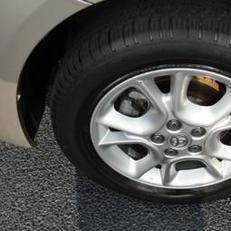
\includegraphics[width=0.3\textwidth]{figures/train00368.jpg}}
	\subfigure[Tire (label = 4)]{\label{fig:tire}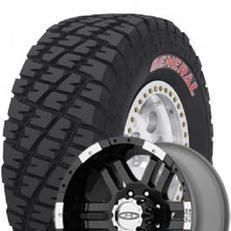
\includegraphics[width=0.3\textwidth]{figures/train00942.jpg}}
	\subfigure[Another car (label = 2)]{\label{fig:car}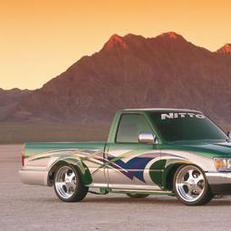
\includegraphics[width=0.3\textwidth]{figures/train04139.jpg}}
	\caption{Some samples from the training set}
\end{figure}

\section{Data Description}

We have to design a system to classify images based on the object depicted.
There are 4 classes: the image can contain an airplane, a car, a horse or neither of them.

The training set consists of either color or gray-scale images of size 231x231. It contains 6000 images. Each image is labeled and assotiated with two sets of features: the HOG and the OverFeat ImageNet CNN Features.
Out of these 6000 images there are 964 airplanes, 1162 cars, 1492 horses and 2382 other objects.
Unfortunately, we do not know whether the testing data follows the same distribution.

For acceleration of the experiments, we considered the ways to reduce the number of features. 
One way is to scale down the input images. However, this affects only the HOG features, as CNN represents the neural network weights and does not depend on the number of pixels in the image. We used then the decreased HOG feature array for our SVM classifier to debug the algorithms that otherwise take a long time. On the down side, when we applied them to the original feature they required expensive recalibration.

The CNN feature array seems very sparse. However an investigation shown that each feature (except for the last one) is nonzero for at least 20 images in the training set. There is no point in looking for corelated features as the number of dimensions(36865) by far exceeds the number of data points(6000) so most of them are dependent.

\paragraph{Training data}

We do not find any common structure for a horse, a car or an airplane, so it is reasonable to do binary prediction based on the multiclass prediction. Simply:
$y_{binary} = (y_{multiclass} \neq 4)$  -- if the classifier did not recognize any of the three classes we have the ``Other'' picture. Here $y_{multiclass} = index\ of(1, [y_{airplane}, y_{car}, y_{horse}])$, and $y_{airplane}$, $y_{car}$ and $y_{horse}$ are computed with a binary classifier.

The problem may arise for disputed cases (e.g. $y_{horse} == 1$ and $y_{car} == 1$). We may train 3 additional One-to-One classifiers for each of those, if we get enough cases for it.

\subsection{Features description}
\paragraph{HOG feature} HOG is widely use in computer vision. 
The basic idea is that the shape and appearance of an object is often well characterized by the distribution of local intensity gradients or edge directions \cite{hog}. It greatly reduces the illumination, color and orientation effects on the images.
Figure \ref{fig:image_car} and \ref{fig:hog} shows respectively an image form the training set and a visualization of its HOG feature.
And in fact, the shape of the car is recognizable even by a human in the HOG visualization. Another evidence that HOG preserves most of the necessary information is the Inverse HOG algorithm\cite{vondrick2015visualizing} that reconstructs the image, based on the HOG feature. The same paper shows that in some cases HOG is not sufficient to interpret the image no matter which ML algorithm you use.

\paragraph{CNN features} Features extracted from the OverFeat convolutional neural network (CNN). These are the outputs of individual predictors that each learned to identify some specific property or element of the image.

\begin{figure}[!t]
	\centering
	\subfigure[Training image]{\label{fig:image_car}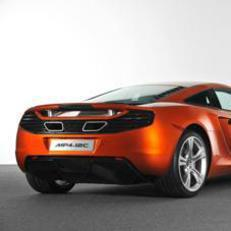
\includegraphics[width=0.4\textwidth]{figures/train00003.jpg}}
	\hspace{10pt}
	\subfigure[HOG feature]{\label{fig:hog}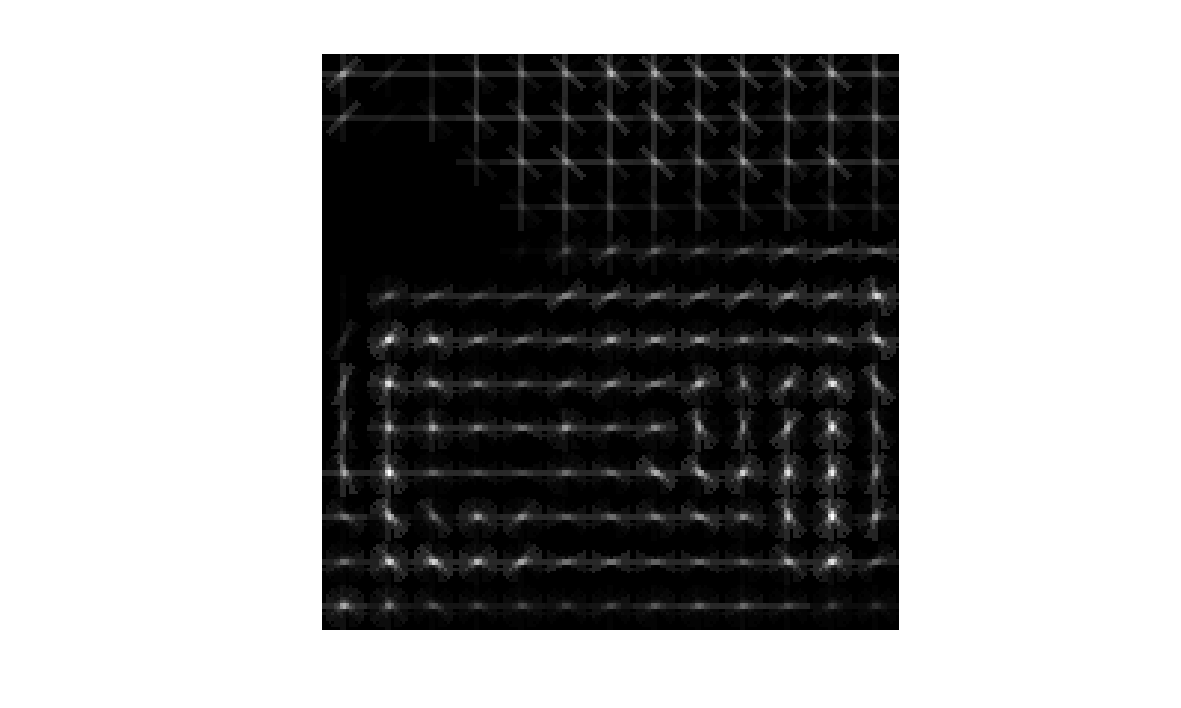
\includegraphics[width=0.4\textwidth]{figures/hog.pdf}}
	\caption{Visualization of the HOG feature}
\end{figure}

The test set contains only the HOG and CNN features and not the original images.
As a consequence we should focus on optimizing the classification based on these two sets of features and not try to find and extract a better one.
The test set contains 11'453 samples.

\section{Predict test data}

This section describes the four different Machine Learning (ML) methods and models that used to classify the images. 
First we detail the performance measure, then the classification methods.
We experimented with both binary and multiclass classification.
We chose to focus on multiclass classification, and then derive the binary predictions.


\subsection{Cross-Validation}

K-fold and Balanced Error Rate (BER) are used to measure the performance of the classification methods.
K-fold returns an unbiased estimate of the error by randomly partitioning the data into K groups of the same size, training a classifier on K-1 group and testing the model on the remaining one. This process is repeated with each of the K groups being the test one. %<-- stopped here.
The parameter K is not easy to set for this project. 
We want a K that split the training and testing set with a good proportion, that is there is enough data in the training set to train a neural network, SVM or a random forest while at the same time having a testing set large enough to estimate the BER.
A problem here is that for each fold we have to train the model, which is time consuming. 
We used a K equal to 3, because for larger K we waste too much time training the model.

\subsection{Convolutional Neural Network}
The file named \emph{imageClassificationExample.m} given in the project website use a simple neural network (NN) from the \emph{DeepLearnToolbox}.
In the example, this NN is trained on the HOG features and give a BER of 30\% with 3-Fold Cross validation. Note that the others parameters are still set to their default values, that is the number of epochs is 20, the batch size 100, the learning rate 2.

We tried to train the NN with the CNN features and the same parameters, and this time the BER is 13\%.
The next step is trying to find optimal values for the parameters with a grid search. As the NN takes quite a long time to train, we cannot afford to do a grid search with too many parameters.
We obtain the best performance with a learning rate = 3, number of epoch = 90 and batch size = 200. 
Figure \ref{tbl:errClassNN} shows the results. The overall BER is $\dfrac{1}{C}\sum Class BER= 12\%$ . 

Lastly, we modify the NN to handle binary classification. This time it predicts if an object is in the set $\{Airplane, Car, Horse\}$ or not. The BER with the same parameters as before is 11\%.

\begin{table}
	\centering
	\begin{tabular}{|c|c|c|c|c|c|c|}
		\hline Class & $N_{c}$ & Airplane & Car & Horse & Other & Class BER \\ 
		\hline Airplane	  & 323 & 285 & 11 & 3 & 24 & 12 ($\pm$ 1)\% \\ 
		\hline Car			& 383 & 7 & 352 & 0 & 24 &  8 ($\pm$ 2)\% \\ 
		\hline Horse      & 513 & 4 & 2 & 450 & 57 &  14 ($\pm$ 2)\% \\ 
		\hline Other      & 781 & 20 & 16 & 54 & 691 & 12 ($\pm$ 1) \% \\ 
		\hline 
	\end{tabular} 
	\caption{Predictions error of Multi-class NN for each class}
	\label{tbl:errClassNN}
\end{table}

\subsection{Random Forests}
We saw in class that Random Forests (RF) are one of the last technique capable to compete with Neural Networks.
As a consequence, we chose to experiment with them to try to outperform our firsts results.

Random forests choose randomly a subset of input variables to build many trees and reduce the variance of the output by taking the average of many outputs.

Here we use the Matlab function named \emph{TreeBagger}. We set the number of trees to 300, this value was determined with grid search.
We obtain a BER of 13\% with 3-fold cross validation. Table \ref{tbl:errClassNotBal} shows the predictions error for each class. Take the first line as example. The true class is Airplane and there is $N_c$ sample in it. The following columns show what the random forest predicted.
Here we notice that most of the samples that are misclassified are put in the categorie "Other" when they actually belong to another one.
This is maybe because of the class imbalance during the training of the model. Indeed we mention earlier that there are 6000 images: 964 airplanes, 1162 cars, 1492 horses and 2382 other objects.

The next step is to create the decision trees with a balanced training set. Ideally we want to add images in the classes with less samples so we increase the size of the training set.
Here adding hundreds of new images would definitely violate the 20MB size constraints, so instead we reduced the size of the training set by randomly deleting sample in the classes with more data. 
We end up with a training set containing 964 images for each class, so a total of 3856 images. 
We obtain a BER of 10\%. Table \ref{tbl:errClassBal} shows the BER for each class.

\begin{table}[!htb]
	\centering
		\begin{tabular}{|c|c|c|c|c|c|c|}
			\hline Class & $N_{c}$ & Airplane & Car & Horse & Other & Class BER \\ 
			\hline Airplane    & 322 & 259 & 16 & 1 & 46 & 20 ($\pm$ 1)\% \\ 
			\hline Car 			 & 382 & 1 & 356 & 2 & 23 & 6 ($\pm$ 1)\% \\ 
			\hline Horse       & 489 & 0 & 1 & 393 & 95 & 19 ($\pm$ 1)\% \\ 
			\hline Other       & 807 & 6 & 9 & 35 & 757 & 6 ($\pm$ 1)\% \\ 
			\hline 
		\end{tabular} 
		\caption{Predictions error of random forests for each class with unbalanced training set}
		\label{tbl:errClassNotBal}
\end{table}

\begin{table}
	\centering
	\begin{tabular}{|c|c|c|c|c|c|c|}
		\hline Class 		 & $N_{c}$ & Airplane & Car & Horse & Other & Class BER \\ 
		\hline Airplane 	& 328 & 303 & 8 & 0 & 17 & 8 ($\pm$ 1)\% \\ 
		\hline Car 			  & 329 & 6 & 312 & 3 & 8 & 4 ($\pm$ 1)\% \\ 
		\hline Horse		& 324 & 2 & 0 & 299 & 23 & 8 ($\pm$ 1)\% \\ 
		\hline Other 	    & 304 & 16 & 6 & 37 & 245 & 20 ($\pm$ 1)\% \\ 
		\hline 
	\end{tabular} 
	\caption{Predictions error of random forests for each class with balanced training set}
	\label{tbl:errClassBal}
\end{table}


\subsection{SVM}

We use One-vs-All scheme, because the time at our disposal is insufficient to train and tweak the One-vs-One SVM. The miss-prediction rates for each binary classifier are shown in the Table \ref{tbl:SVMerr}. We use HOG features for this method, as it is known to give good results \cite{zhang2010pedestrian}. Unlike the results of Foody\&Co. \cite{foody2004relative}, the performance of our SVM model is the worst amongst the tried approaches. Big difference between train and test errors suggests that the model overfit. No wonder, the number of features is bigger than the number of training data points. To overcome this problem we tried:

\paragraph{Feature-reduction} We computed the median histogram, summarizing histograms for all the cells, therefore decreasing the number of features to just 32 numbers. Unfortunately, this transformation loses too much information, so we were unable to improve the performance of SVM with this reduced feature.

\paragraph{Hard negative mining} A cheap way to expand the training set is to add the slightly-shaked negative images which cause misspredictions. This helps eliminate false positives improving the overal precision of the classifier, although it requires recalibration of the SVM parameters. Unfortunately, as you can see from the Table \ref{tbl:SVMerr}, it also did not help much.

We chose optimal parameters using a manual form of coordinate descent, applying cross validation to a number of candidate values. Since the computation for each point takes a long time, we could not reach the strict optimum, but judging by the shape of the curve, e.g. Figure \ref{fig:SVMKernelScaleBER}, we got close enough.

\begin{table}
  \centering
  \begin{tabular}{|l|r|r|}
    \hline
    Class & CV BER & CV BER with additional negative samples \\ \hline
    Airplane & 11 ($\pm$ 2) \% & 10 ($\pm$ 1) \% \\
    Car & 9 ($\pm$ 2) \% & 9 ($\pm$ 2) \% \\
    Horse & 15 ($\pm$ 2) \% & 15 ($\pm$ 2) \% \\
    \hline
  \end{tabular}
  \caption{Prediction error for each class for SVM with and without hard-negative mined samples}
  \label{tbl:SVMerr}
\end{table}


\begin{figure}[!t]
  \centering
  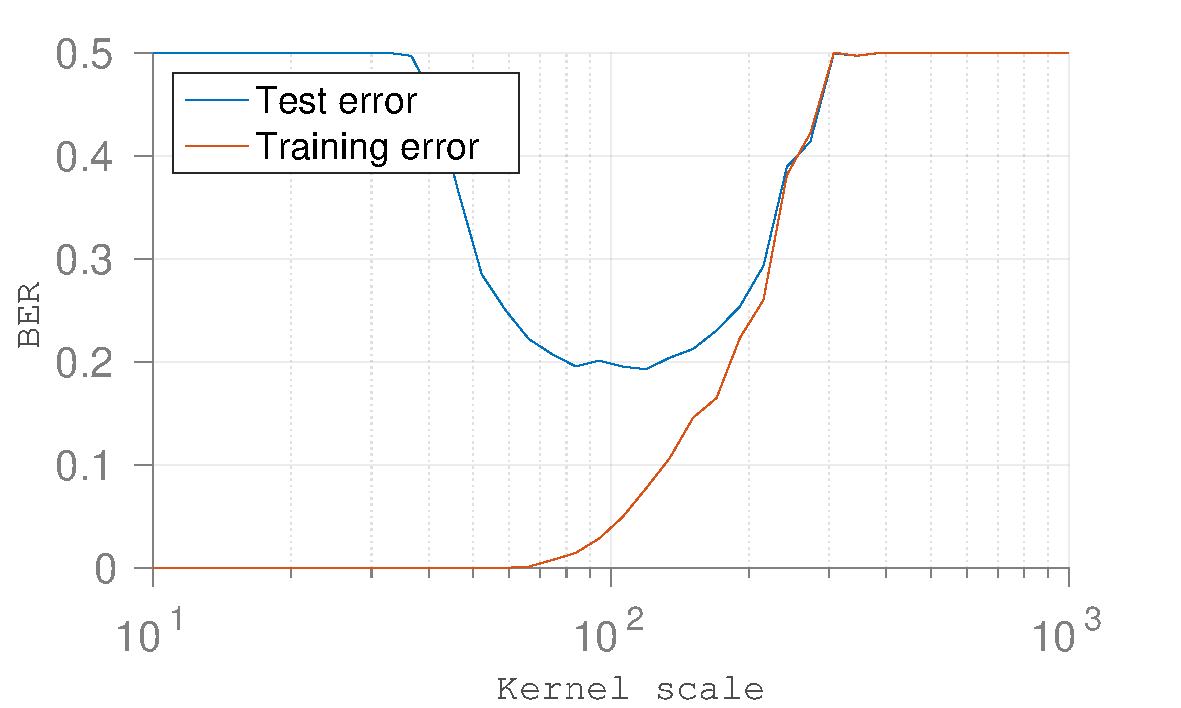
\includegraphics[width=0.9\textwidth]{figures/kernel_scale_ber.pdf}
  \caption{Dependency of train and test BER on the Scale of the SVM kernel.}
  \label{fig:SVMKernelScaleBER}
\end{figure}

\subsection{Ensemble Classifier}

On top of the three classifiers, described above, we implemented an ensemble classifier. It uses the majority vote, with the-most-confident-wins fallback. We expect it to perform at least as the best of the three comprising classifiers. The training of all the models takes a long time on the available resources. Therefore, we are not able to directly measure the precision of the combined predictor, as we did for its components.

We estimate the expected multiclass prediction error for the classifier with the following formula:
\[
BER_{ensemble} = \sum_C weight_C*min(BER_{SVM}^C, BER_{NN}^C, BER_{RF}^C)
\]
Where $C$ iterates over all classes, and $weight_C$ is the predicted fraction of images belonging to that class on the test dataset. The calculated value is $BER_{ensemble} \approx 7\%$.

\section{Implementation Details}

We implemented the multiclass SVM classifier, and an Ensemble classifier on top of the three trained classifiers: Neural Networks, Random Forest with CNN, and SVM with HOG feature.


\section{Summary}

In this report we described the methods used to build the image recognition system. 
Neural networks, random forests and SVM are trained and tuned individually so that they offer a performance as good as possible.
Finally we combine those three methods to come up with the binary and multiclass predictions we have to submit. 
With this association the system can improve its performance.

We can take several other directions to keep improving the performance of the system.
For example, other toolboxes should be tested. The neural network given for this lab is outdated and no longer maintained as stated in their website \cite{deeplearningtoolbox}. Other alternatives are suggested: Theano, torch or tensorflow. It is a path that is definitely worth exploring.

Another alternative to improve performance is to enhanced the training set. 
For this project we received 6000 training images, and when we create a balanced dataset, there are only 3856 left.
If the neural network is trained with more images, it can improve its performance.

SVM, clearly needs more training images as well. We could tackle the dimensionality problem by using less buckets, but in this case it is not feasible, as we are not given the images themselves, only the precomputed features.

\bibliographystyle{plain}
\bibliography{References.bib}

\end{document}
